% This file is generated by the MATLAB m-file laprint.m. It can be included
% into LaTeX documents using the packages graphicx, color and psfrag.
% It is accompanied by a postscript file. A sample LaTeX file is:
%    \documentclass{article}\usepackage{graphicx,color,psfrag}
%    \begin{document}% This file is generated by the MATLAB m-file laprint.m. It can be included
% into LaTeX documents using the packages graphicx, color and psfrag.
% It is accompanied by a postscript file. A sample LaTeX file is:
%    \documentclass{article}\usepackage{graphicx,color,psfrag}
%    \begin{document}% This file is generated by the MATLAB m-file laprint.m. It can be included
% into LaTeX documents using the packages graphicx, color and psfrag.
% It is accompanied by a postscript file. A sample LaTeX file is:
%    \documentclass{article}\usepackage{graphicx,color,psfrag}
%    \begin{document}% This file is generated by the MATLAB m-file laprint.m. It can be included
% into LaTeX documents using the packages graphicx, color and psfrag.
% It is accompanied by a postscript file. A sample LaTeX file is:
%    \documentclass{article}\usepackage{graphicx,color,psfrag}
%    \begin{document}\input{N_peri}\end{document}
% See http://www.mathworks.de/matlabcentral/fileexchange/loadFile.do?objectId=4638
% for recent versions of laprint.m.
%
% created by:           LaPrint version 3.16 (13.9.2004)
% created on:           27-Jun-2011 10:51:34
% eps bounding box:     15 cm x 11.25 cm
% comment:              
%
\begin{psfrags}%
\psfragscanon%
%
% text strings:
\psfrag{s03}[t][t]{\color[rgb]{0,0,0}\setlength{\tabcolsep}{0pt}\begin{tabular}{c}{\Large $a/M$}\end{tabular}}%
\psfrag{s04}[b][b]{\color[rgb]{0,0,0}\setlength{\tabcolsep}{0pt}\begin{tabular}{c}{\Large $r_\mathrm{p}/M$}\end{tabular}}%
%
% xticklabels:
\psfrag{x01}[t][t]{$-1.0$}%
\psfrag{x02}[t][t]{$-0.8$}%
\psfrag{x03}[t][t]{$-0.6$}%
\psfrag{x04}[t][t]{$-0.4$}%
\psfrag{x05}[t][t]{$-0.2$}%
\psfrag{x06}[t][t]{$0.0$}%
\psfrag{x07}[t][t]{$0.2$}%
\psfrag{x08}[t][t]{$0.4$}%
\psfrag{x09}[t][t]{$0.6$}%
\psfrag{x10}[t][t]{$0.8$}%
\psfrag{x11}[t][t]{$1.0$}%
%
% yticklabels:
\psfrag{v01}[r][r]{$13$}%
\psfrag{v02}[r][r]{$14$}%
\psfrag{v03}[r][r]{$15$}%
\psfrag{v04}[r][r]{$16$}%
\psfrag{v05}[r][r]{$17$}%
\psfrag{v06}[r][r]{$18$}%
\psfrag{v07}[r][r]{$19$}%
\psfrag{v08}[r][r]{$20$}%
\psfrag{v09}[r][r]{$21$}%
\psfrag{v10}[r][r]{$22$}%
%
% Figure:
\resizebox{12cm}{!}{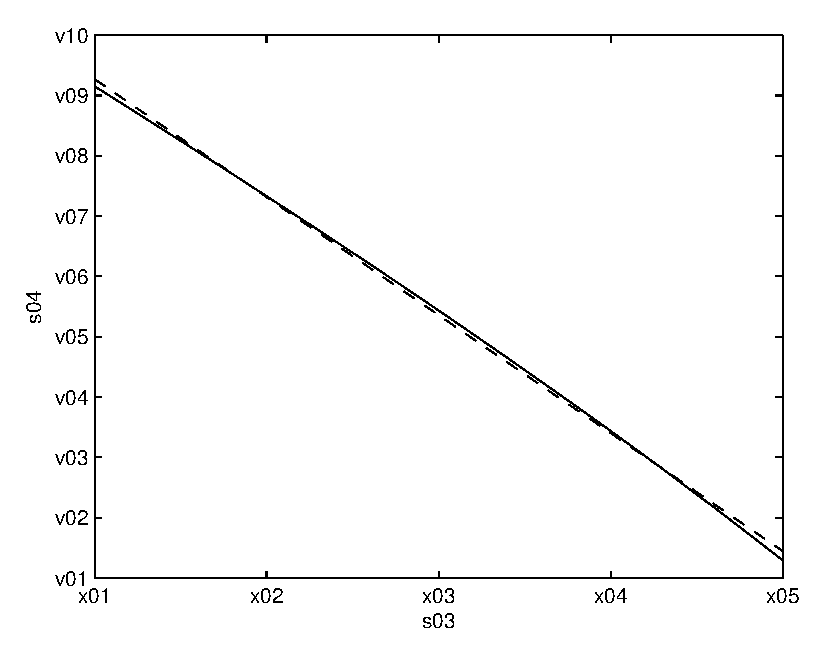
\includegraphics{N_peri.eps}}%
\end{psfrags}%
%
% End N_peri.tex
\end{document}
% See http://www.mathworks.de/matlabcentral/fileexchange/loadFile.do?objectId=4638
% for recent versions of laprint.m.
%
% created by:           LaPrint version 3.16 (13.9.2004)
% created on:           27-Jun-2011 10:51:34
% eps bounding box:     15 cm x 11.25 cm
% comment:              
%
\begin{psfrags}%
\psfragscanon%
%
% text strings:
\psfrag{s03}[t][t]{\color[rgb]{0,0,0}\setlength{\tabcolsep}{0pt}\begin{tabular}{c}{\Large $a/M$}\end{tabular}}%
\psfrag{s04}[b][b]{\color[rgb]{0,0,0}\setlength{\tabcolsep}{0pt}\begin{tabular}{c}{\Large $r_\mathrm{p}/M$}\end{tabular}}%
%
% xticklabels:
\psfrag{x01}[t][t]{$-1.0$}%
\psfrag{x02}[t][t]{$-0.8$}%
\psfrag{x03}[t][t]{$-0.6$}%
\psfrag{x04}[t][t]{$-0.4$}%
\psfrag{x05}[t][t]{$-0.2$}%
\psfrag{x06}[t][t]{$0.0$}%
\psfrag{x07}[t][t]{$0.2$}%
\psfrag{x08}[t][t]{$0.4$}%
\psfrag{x09}[t][t]{$0.6$}%
\psfrag{x10}[t][t]{$0.8$}%
\psfrag{x11}[t][t]{$1.0$}%
%
% yticklabels:
\psfrag{v01}[r][r]{$13$}%
\psfrag{v02}[r][r]{$14$}%
\psfrag{v03}[r][r]{$15$}%
\psfrag{v04}[r][r]{$16$}%
\psfrag{v05}[r][r]{$17$}%
\psfrag{v06}[r][r]{$18$}%
\psfrag{v07}[r][r]{$19$}%
\psfrag{v08}[r][r]{$20$}%
\psfrag{v09}[r][r]{$21$}%
\psfrag{v10}[r][r]{$22$}%
%
% Figure:
\resizebox{12cm}{!}{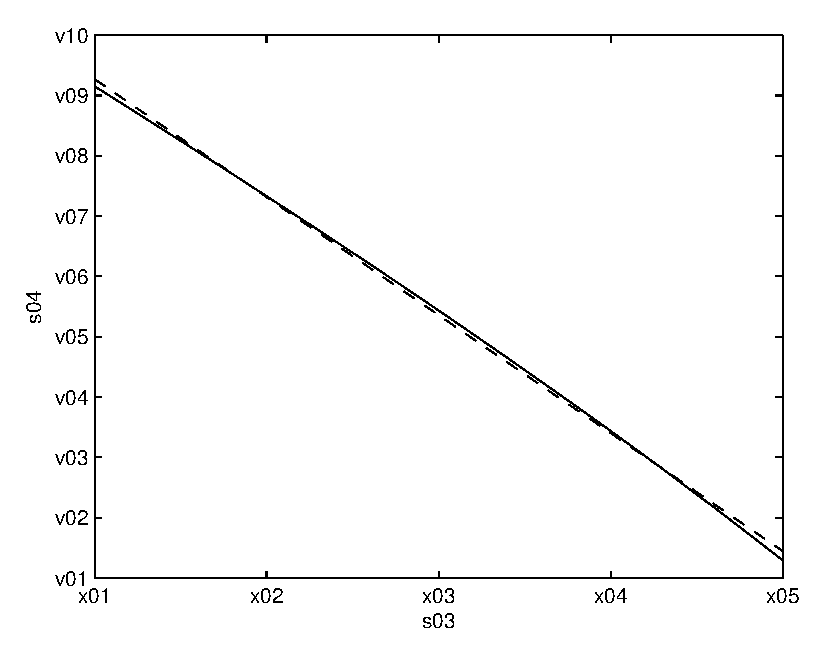
\includegraphics{N_peri.eps}}%
\end{psfrags}%
%
% End N_peri.tex
\end{document}
% See http://www.mathworks.de/matlabcentral/fileexchange/loadFile.do?objectId=4638
% for recent versions of laprint.m.
%
% created by:           LaPrint version 3.16 (13.9.2004)
% created on:           27-Jun-2011 10:51:34
% eps bounding box:     15 cm x 11.25 cm
% comment:              
%
\begin{psfrags}%
\psfragscanon%
%
% text strings:
\psfrag{s03}[t][t]{\color[rgb]{0,0,0}\setlength{\tabcolsep}{0pt}\begin{tabular}{c}{\Large $a/M$}\end{tabular}}%
\psfrag{s04}[b][b]{\color[rgb]{0,0,0}\setlength{\tabcolsep}{0pt}\begin{tabular}{c}{\Large $r_\mathrm{p}/M$}\end{tabular}}%
%
% xticklabels:
\psfrag{x01}[t][t]{$-1.0$}%
\psfrag{x02}[t][t]{$-0.8$}%
\psfrag{x03}[t][t]{$-0.6$}%
\psfrag{x04}[t][t]{$-0.4$}%
\psfrag{x05}[t][t]{$-0.2$}%
\psfrag{x06}[t][t]{$0.0$}%
\psfrag{x07}[t][t]{$0.2$}%
\psfrag{x08}[t][t]{$0.4$}%
\psfrag{x09}[t][t]{$0.6$}%
\psfrag{x10}[t][t]{$0.8$}%
\psfrag{x11}[t][t]{$1.0$}%
%
% yticklabels:
\psfrag{v01}[r][r]{$13$}%
\psfrag{v02}[r][r]{$14$}%
\psfrag{v03}[r][r]{$15$}%
\psfrag{v04}[r][r]{$16$}%
\psfrag{v05}[r][r]{$17$}%
\psfrag{v06}[r][r]{$18$}%
\psfrag{v07}[r][r]{$19$}%
\psfrag{v08}[r][r]{$20$}%
\psfrag{v09}[r][r]{$21$}%
\psfrag{v10}[r][r]{$22$}%
%
% Figure:
\resizebox{12cm}{!}{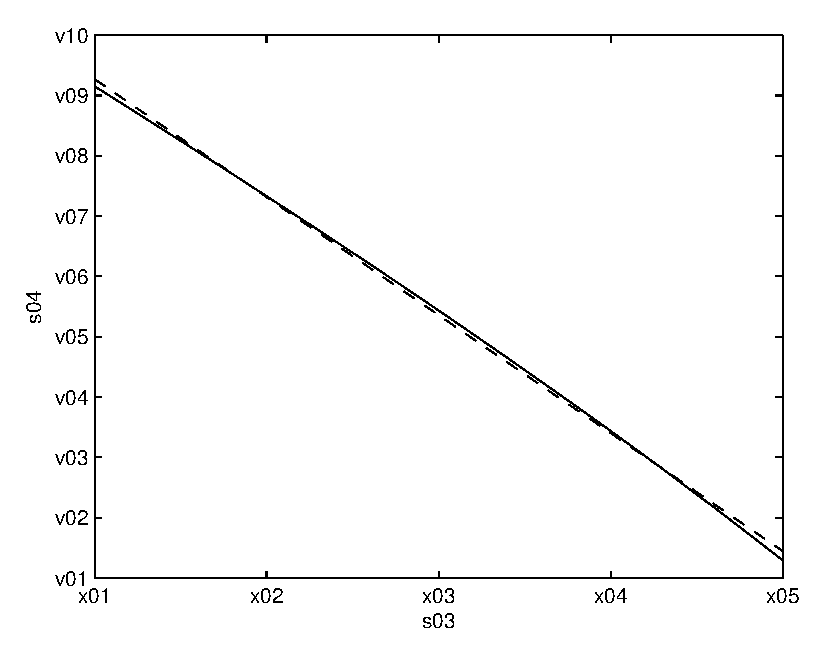
\includegraphics{N_peri.eps}}%
\end{psfrags}%
%
% End N_peri.tex
\end{document}
% See http://www.mathworks.de/matlabcentral/fileexchange/loadFile.do?objectId=4638
% for recent versions of laprint.m.
%
% created by:           LaPrint version 3.16 (13.9.2004)
% created on:           27-Jun-2011 10:51:34
% eps bounding box:     15 cm x 11.25 cm
% comment:              
%
\begin{psfrags}%
\psfragscanon%
%
% text strings:
\psfrag{s03}[t][t]{\color[rgb]{0,0,0}\setlength{\tabcolsep}{0pt}\begin{tabular}{c}{\Large $a/M$}\end{tabular}}%
\psfrag{s04}[b][b]{\color[rgb]{0,0,0}\setlength{\tabcolsep}{0pt}\begin{tabular}{c}{\Large $r_\mathrm{p}/M$}\end{tabular}}%
%
% xticklabels:
\psfrag{x01}[t][t]{$-1.0$}%
\psfrag{x02}[t][t]{$-0.8$}%
\psfrag{x03}[t][t]{$-0.6$}%
\psfrag{x04}[t][t]{$-0.4$}%
\psfrag{x05}[t][t]{$-0.2$}%
\psfrag{x06}[t][t]{$0.0$}%
\psfrag{x07}[t][t]{$0.2$}%
\psfrag{x08}[t][t]{$0.4$}%
\psfrag{x09}[t][t]{$0.6$}%
\psfrag{x10}[t][t]{$0.8$}%
\psfrag{x11}[t][t]{$1.0$}%
%
% yticklabels:
\psfrag{v01}[r][r]{$13$}%
\psfrag{v02}[r][r]{$14$}%
\psfrag{v03}[r][r]{$15$}%
\psfrag{v04}[r][r]{$16$}%
\psfrag{v05}[r][r]{$17$}%
\psfrag{v06}[r][r]{$18$}%
\psfrag{v07}[r][r]{$19$}%
\psfrag{v08}[r][r]{$20$}%
\psfrag{v09}[r][r]{$21$}%
\psfrag{v10}[r][r]{$22$}%
%
% Figure:
\resizebox{12cm}{!}{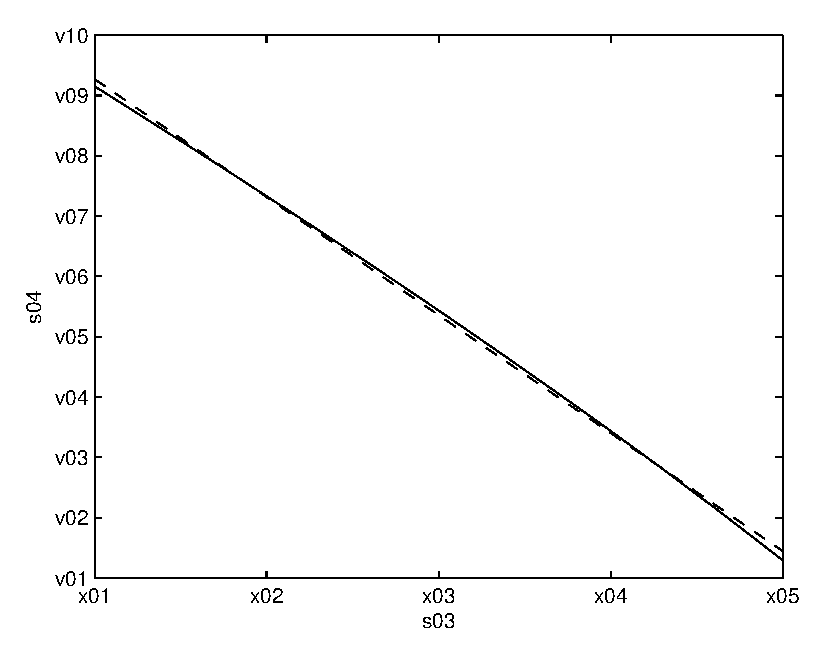
\includegraphics{N_peri.eps}}%
\end{psfrags}%
%
% End N_peri.tex
